
    \mysection{Sacraments}{arcana-seven-sacraments}

    The Seven Sacraments are invoked by Mystics through the \mylink{Gift of Grace}{mystic-virtue-grace}


  \begin{center}
  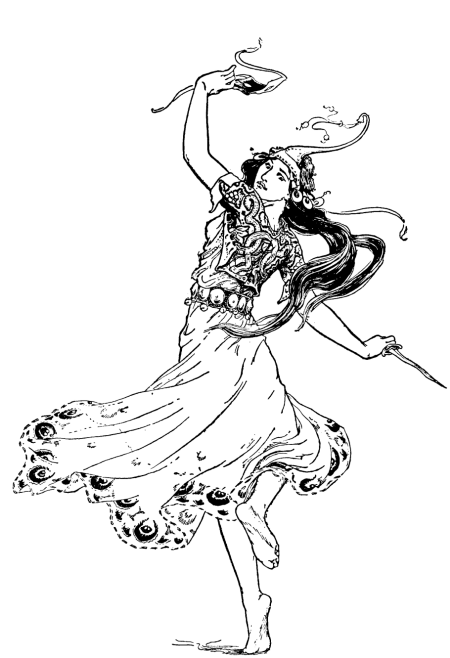
\includegraphics[scale=.5]{Sacraments}
  \end{center}


    \SACRAMENT [
      Name=Bless,
      Link=mystic-sacrament-bless,
      Paradigm=Grace,
      Save=N,
      Duration=Session,
      Counter=None,
      Keywords=Splittable,
      Target=Close Ally or object
    ]

    Choose one unique effect per Grace die invested: 
    1. The Ally can automatically make a single Save roll;
    2. The Ally can automatically succeed on a single \RO or \RS check;
    3. The Ally can immediately end a Markovian duration affecting them;
    4. The Ally or object is Hallowed for the remainder of the Session (this negates the detriment Unhallowed)

    Once an effect is used, it disappears (though the Blessing can be recast)

    \SACRAMENT [
      Name=Consecrate,
      Link=mystic-sacrament-consecrate,
      Paradigm=Grace,
      Save=N,
      Duration=Concentration,
      Counter=None,
      Keywords=None,
      Target=Close radius
    ]

    You exude a \DICE meter diameter circle of \mylink{Hallowed Ground}{miracle-hallowed-ground} around yourself. You cannot move or be carried while concentrating on this Sacrament.

    Note that the area of Hallowed Ground will temporarily cancel out the effects of \mylink{Unhallowed Earth}{occultism-unhallowed-earth} (making it "normal"), but that Sacraments cannot be performed while you are on Unhallowed Earth.

   \SACRAMENT [
      Name=Curse the Unhallowed,
      Link=mystic-sacrament-curse-the-unhallowed,
      Paradigm=Grace,
      Save=Y,
      Duration=0,
      Counter=None,
      Keywords=Splittable,
      Target=\DICE Nearby Unhallowed
    ]


    Up to \DICE Unhallowed creatures take \SUMDICE + \DICE damage (Save for half).  You can divide this damage up any way you like.

    \example {
      Oberlan Xi, Mystic of Pilzesser, performs the sacrament of Curse the Unhallowed on a ghoul and a group of skeletons. He rolls 3 d4 Grace dice in the attempt and gets a 9 - adding the number of \DICE he rolled, this becomes a 12 (9+3).  He can affect up to 3 creatures, and decides to deal 6 damage to the ghoul and 3 damage to two of the skeletons (he could also have just dealt 12 damage to the ghoul if he preferred).
    }  


    \SACRAMENT [
      Name=Heal,
      Link=mystic-sacrament-lay-on-hands,
      Paradigm=Grace,
      Save=N,
      Duration=Concentration,
      Counter=None,
      Keywords=None,
      Target=Close (touch) Allies
    ]

    Heal up to \SUMDICE points of Flesh by touch. You may distribute healing among as many creatures as you would like, as long as the total Flesh healed does not exceed \SUMDICE and you maintain concentration. If you invest 4 \DICE or more, you may instead heal a single target's Flesh fully






   \SACRAMENT [
      Name=Loaves and Fishes,
      Link=mystic-sacrament-loaves-and-fishes,
      Paradigm=Grace,
      Save=N,
      Duration=0,
      Counter=None,
      Keywords=None,
      Target=Close radius
    ]


    You create enough food to feed \SUMDICE people for one meal, along with clean water to fill one mug per person. Mugs, utensils, and condiments are not provided.  Those that participate in the meal do not need to roll Provisions for a Bivouac.  

    \SACRAMENT [
      Name=Meditation,
      Link=mystic-sacrament-meditation,
      Paradigm=Grace,
      Save=N,
      Duration=0,
      Counter=None,
      Keywords=0,
      Target=Self
    ]

    You drop into deep meditation.  It needs to be quiet-ish, so you can't do it during Combat.  You can do up to \DICE of the following (you can only choose each option once per Meditation):
    \mylist {
        \item a) Heal 1 \UD of damage to an Intangible Stat
        \item b) Roll your \FOC and heal that much Flesh (up to \MAX)
        \item c) Roll your \FOC and heal that much Grit (up to \MAX)
        \item d) Purge yourself of a Toxin
    }


    \cbreak


    \SACRAMENT [
      Name=Walk on Water,
      Link=mystic-sacrament-walk-water,
      Paradigm=Grace,
      Save=N,
      Duration=Concentration,
      Counter=None,
      Keywords=Splittable,
      Target=Self and \DICE-1 Close (touch) Allies
    ]

    You and up to \DICE-1 Allies can slowly walk over water for as long as you maintain Concentration. 

